\documentclass[a4paper, 11pt]{report}
\setcounter{tocdepth}{3}
\usepackage[utf8]{inputenc}
\usepackage[french]{babel}
\usepackage[T1]{fontenc}
\usepackage{graphicx}
\usepackage{xcolor}
\usepackage{booktabs}
\usepackage{tabularx}
\usepackage{fourier} 
\usepackage{array}
\usepackage{makecell}
\usepackage[top=2.5cm,bottom=2.5cm,right=2.5cm,left=2.5cm]{geometry}
\usepackage{amsmath}
\usepackage{xcolor}
\usepackage{colortbl,hhline}
\usepackage{subfig}
\usepackage{multirow}
\usepackage{comment}
\usepackage{makecell}

\usepackage{algorithmic,algorithm}


\usepackage{array}
\newcolumntype{L}[1]{>{\raggedright\let\newline\\\arraybackslash\hspace{0pt}}m{#1}}
\newcolumntype{C}[1]{>{\centering\let\newline\\\arraybackslash\hspace{0pt}}m{#1}}
\newcolumntype{R}[1]{>{\raggedleft\let\newline\\\arraybackslash\hspace{0pt}}m{#1}}



\renewcommand{\listalgorithmname}{Liste des \ALG@name s}

\definecolor{yacine}{RGB}{241,241,241}
\usepackage{tikz}
\def\checkmark{\tikz\fill[scale=0.4](0,.35) -- (.25,0) -- (1,.7) -- (.25,.15) -- cycle;} 

\usepackage[backend=bibtex,style=numeric,sorting=nty]{biblatex}
\nocite{*} %Ausgabe aller Bibliographieeinträges
\usepackage{hyperref}
\hypersetup{
    linktoc=all,     %set to all if you want both sections and subsections linked
}

\newtheorem{definition}{Definition}
\newcommand{\set}[1]{\ensuremath{\overline{#1}}}
\newcommand{\tupleset}{\ensuremath{\mathcal{T}}}
\newcommand{\arbreset}{\ensuremath{\mathcal{A}}}
\newcommand{\classeset}{\ensuremath{\mathcal{Y}}}
\newcommand{\attributset}{\ensuremath{\mathcal{AT}}}
\newcommand{\valeurset}{\ensuremath{\mathcal{V}}}
\newcommand{\nat}{\ensuremath{\mathbb{N}}}
\newcommand{\real}{\ensuremath{\mathbb{R}}}

\newcommand{\regleset}{\ensuremath{\mathcal{R}}}


\bibliography{biblio2} 
%\usepackage[backend=biber, style=ieee]{biblatex}  
%\addbibresource{bibilographie.bib}
\begin{document}

\begin{chapter}{Les arbres de décision}

\begin{figure}[h!]
\begin{center}
	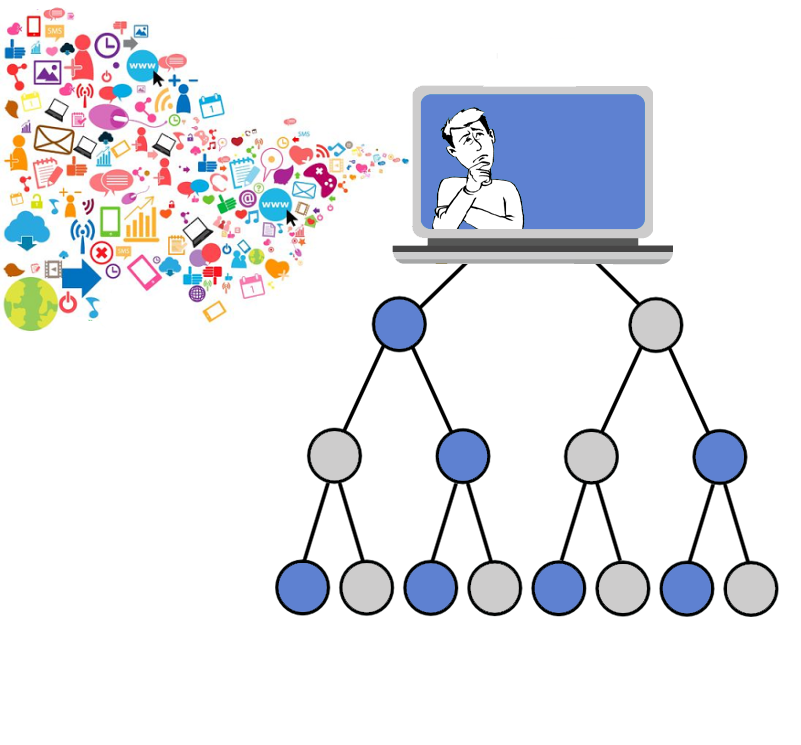
\includegraphics[scale=0.6]{Images/intro3}
	%\caption{ma figure.\label{figure1}}
\end{center}
\end{figure}






\newpage
\tableofcontents
\newpage
%%%%%%%%%%%%%%%%%%%%%%%%%%%
\section{Introduction}
De nos jours, la donnée est tellement importante que le défi n'est pas seulement de la stocker, mais aussi de la traiter, dans le but d'en extraire le maximum de connaissances, aussi bien prédictives que descriptives. Ce processus est appelé \emph{Data Mining}, il englobe beaucoup de techniques, dont les arbres de décision, que nous allons traiter durant ce chapitre, en définissant les notions clés, en présentant quelques algorithmes très utilisés, avec en conclusion, une étude comparative.
\section{Data Mining}
Traduit en fouille ou forage de données, considéré par beaucoup de chercheur comme l’un des sujets de recherche clés dans les systèmes de base de données et d’apprentissage automatique \cite{553155}. 
\\Le \emph{Data Mining} est défini comme étant un ensemble de techniques permettant extraire de la connaissance utile, à partir d'un grand volume de données à l'état brute. 

\begin{figure}[!h]
\begin{center}
	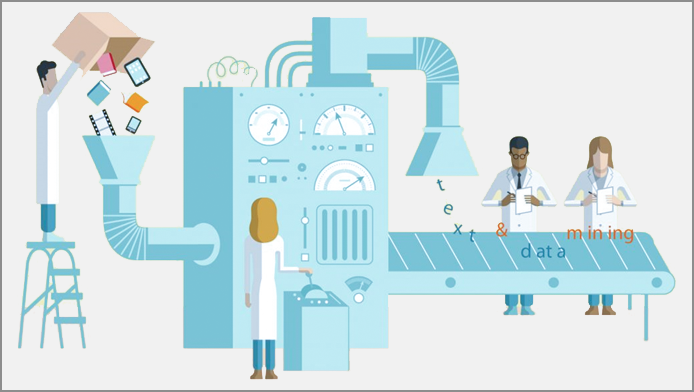
\includegraphics[scale=0.6]{Images/DataMining2.png}
	\caption{Data Mining}
\end{center}
\end{figure}

Le \emph{Data Mining} repose principalement sur des méthodes qui peuvent être classées en deux catégories, la caractéristique utilisée pour cette classification est le fait que la machine, dispose ou non d'un échantillon à apprendre avant la création du modèle.\\

\begin{itemize}
\item Apprentissage supervisé\\
L'idée consiste à se baser sur un ensemble de données d'apprentissage, afin de créer un modèle $Z = (X,Y)$,  en mappant entre un ensemble de variables d'entrée X, et une variable de classe Y. L'application de ce modèle a pour but de prédire, de manière automatique, les classes de nouvelles données \cite{wolpert2002supervised}.\\


Ce type d'apprentissage concerne essentiellement :
\begin{enumerate}
\item La classification : ou la classe à prédire est de type discret
\item La régression : ou la classe à prédire est de type continu
\\Parmi les techniques les plus utilisées d'apprentissage supervisé, nous pouvons citer : 
\begin{itemize}
\item Les réseau de neurones.
\item Les arbres de décision.

\end{itemize}
\end{enumerate}
\newpage
\begin{figure}[!h]
\begin{center}
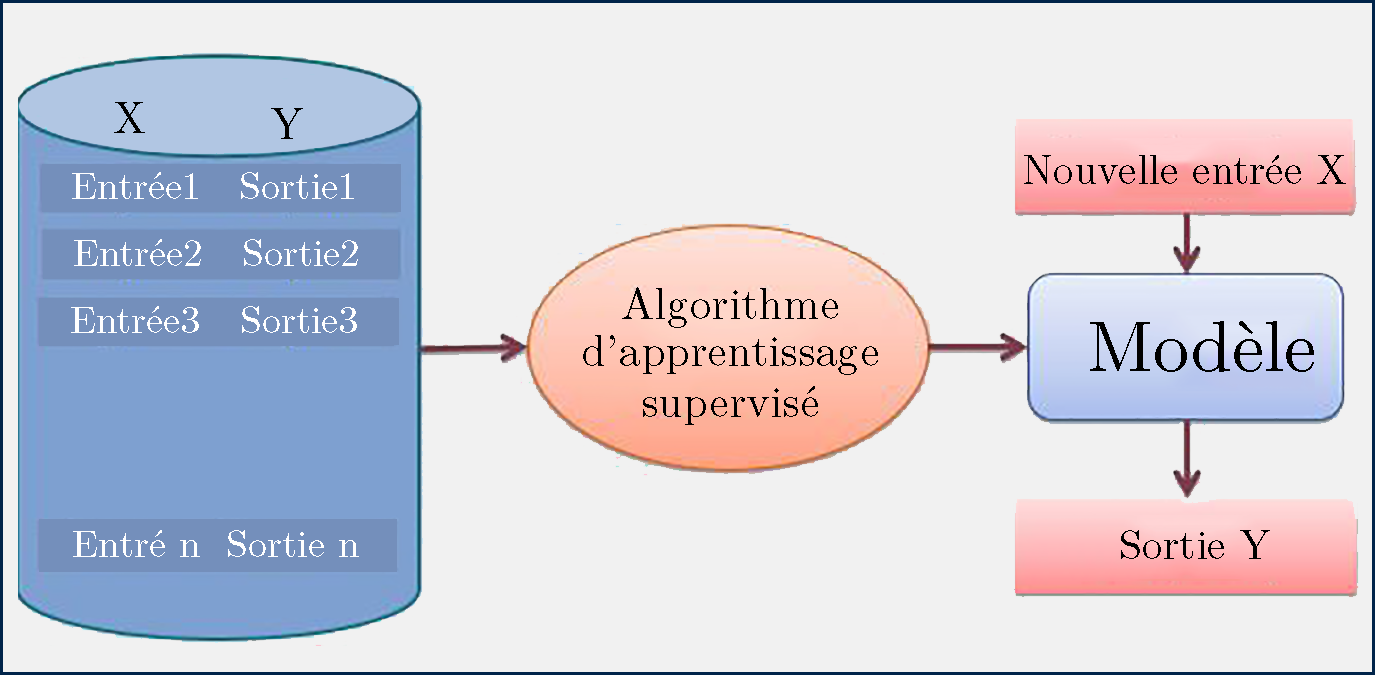
\includegraphics[scale=0.6]{Images/suppervise}
\caption{Apprentissage supervisé}
\end{center}
\end{figure}

\item Apprentissage non supervisé
\\L'apprentissage non supervisé étudie comment les systèmes peuvent apprendre à représenter des schémas d'entrée particuliers d'une manière qui reflète la structure statistique de la collection globale de données\cite{dayan1999unsupervised}, sans se baser sur un modèle crée au préalable.
\\Parmi les techniques d'apprentissage non supervisé, nous pouvons citer :
\begin{itemize}
\item La segmentation : qui, a partir d'un ensemble hétérogène, permet de créer des sous groupe homogènes.
\item Les associations : qui permet de découvrir des association entre les instances d'un tres grand volume de données. Exemple: Les clients qui achètent le produit $P_1$ et $P_2$, achètent aussi $P_3$
\end{itemize}

\end{itemize}
\begin{figure}[h!]
\begin{center}
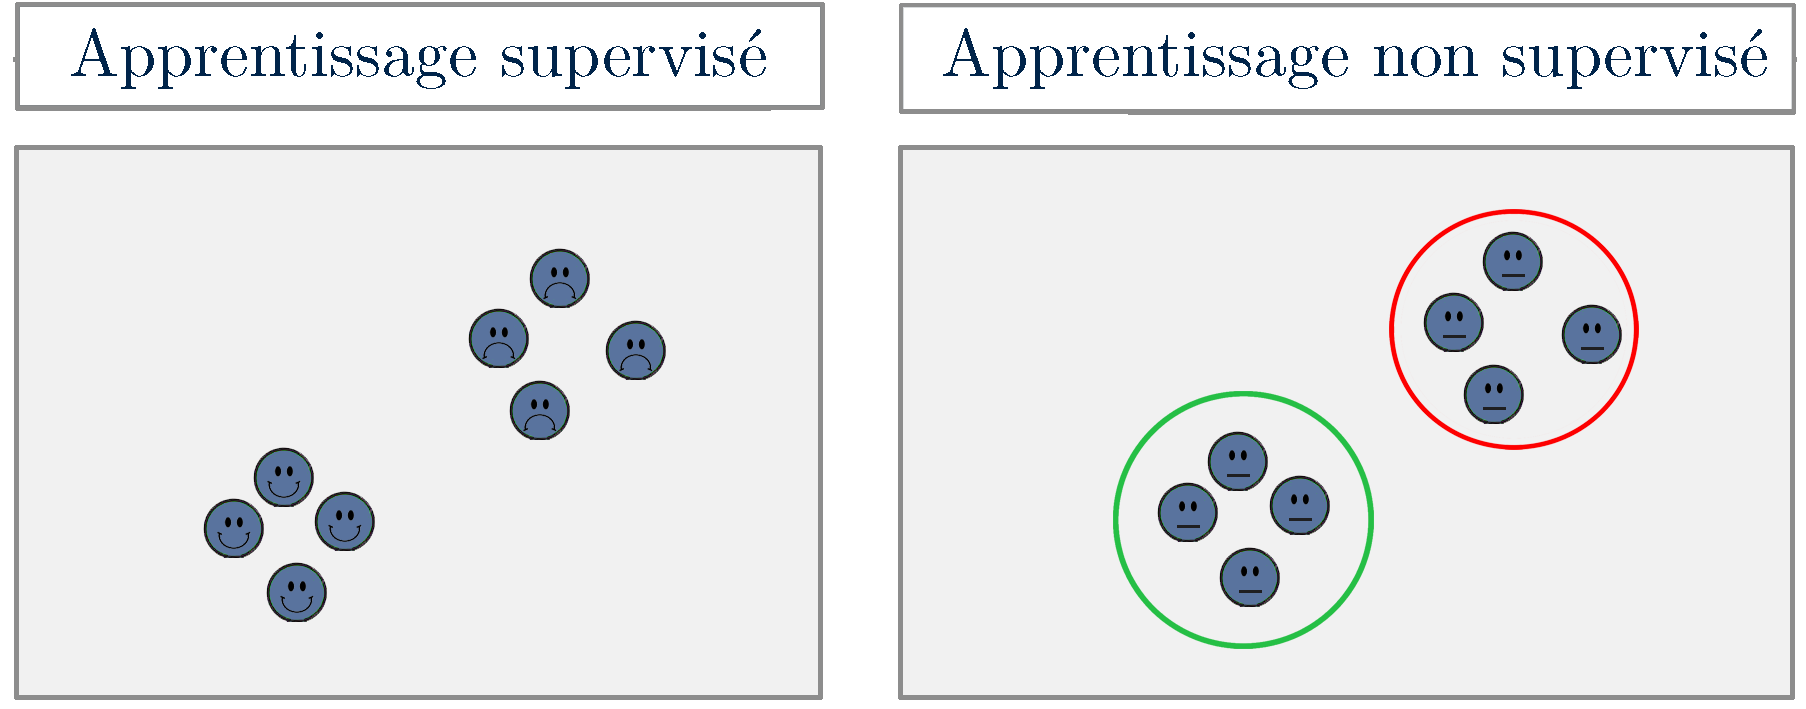
\includegraphics[scale=0.4]{Images/sup_nonsup}
\caption{La différence entre l'apprentissage supervisé et non supervisé}
\end{center}
\end{figure}

%%%%%%%%%%%%%%%%%%%%%%%%%%%%%%%%
\section{Définition}
%%%%%%%%%%%%%%%%%% HISTORIQUE %%%%%%%%%%%%%%%%%%%%%%%%% 
Faisant partie des méthodes de classification supervisées, le but des arbres de décision est aussi de créer un modèle afin de pouvoir classer automatiquement de nouvelles données. La construction de ce modèle se fait à travers des partitions récursives sur l'ensemble de données d'apprentissage, jusqu'à arriver à des sous ensembles homogènes par rapport a la variable de classe. Ainsi, l'ensemble de données d'apprentissage est transformé en un arbre, dans lequel chaque composent a une signification particulière :
\begin{enumerate}
\item Racine : comprend tout l'ensemble de données d'apprentissage. 
\item Nœud interne : représente un test.
\item Nœud terminal (feuille) : représente une décision finale.
\end{enumerate}

\subsection{Formalisation}
\label{sec:formalisation}

Soit $\tupleset$ l'ensemble des tuples possibles, $\valeurset$ l'ensemble des valeurs et $\classeset$ l'ensemble des valeurs de classes.

\begin{definition}[Condition sur un tuple]
  Une condition $C$ est une fonction $\tupleset\rightarrow\{true,false\}$.
\end{definition}

\begin{definition}[Arbre de décision]
  % Soit $\set{X}$ un ensemble d'attributs et $Y$ un attribut.
  L'ensemble des arbres de décision $\arbreset$ est défini inductivement par:
  \begin{itemize}
  \item $Noeud(F)\in\arbreset$ si $F=\{(A_1,C_1),\dots,(A_k,C_k)\}$ tel que les $A_i$ sont des arbres de décisions et les $C_i$ sont des conditions telles que pour tout tuple $t$, il existe un unique $i$ tel que $C_i(t)=true$. 
  \item $Feuille(Y)\in\arbreset$ si $Y\in\classeset$ est une valeur de classe.
  \end{itemize}
\end{definition}

\begin{definition}[Classification locale]
  Soit $A=Noeud(\{(A_1,C_1),\dots,(A_k,C_k)\}$ et soit $t$ un tuple.
  On défini $classificationLocale(A,t)=A_i$ si $i$ est le seul indice tel que $C_i(t)=true$.
\end{definition}


\begin{definition}[Classification par un arbre de décision]
  La classification associée par un arbre de décision $A$ à un tuple $t$ est définie par la fonction $classifie:\arbreset\times\tupleset\rightarrow\classeset$

  $$classifie(A,t)=\left\{
    \begin{array}[c]{ll}
      classifie(A',t)&\textnormal{ si }A=Noeud(F)\textnormal{ et }A' = classificationLocale(A,t)\\
      Y&\textnormal{ si }A=Feuille(Y)
    \end{array}
  \right.
  $$
\end{definition}

\begin{definition}[Equivalence sémantique d'arbres de décision]
  Soient $A_1$ et $A_2$ deux arbres de décision. $A_1$ est sémantiquement équivalent à $A_2$ (noté $A_1\equiv A_2$) si pour tout tuple $t\in\tupleset$, $classification(A_1,t) = classification(A_2,t)$.
\end{definition}

Le rendu du modèle est très aisément interprétable, ce qui fait l'une des principales forces des arbres de décision, comme le montre la figure ci-dessous.

\begin{figure}[!h]
\begin{center}
	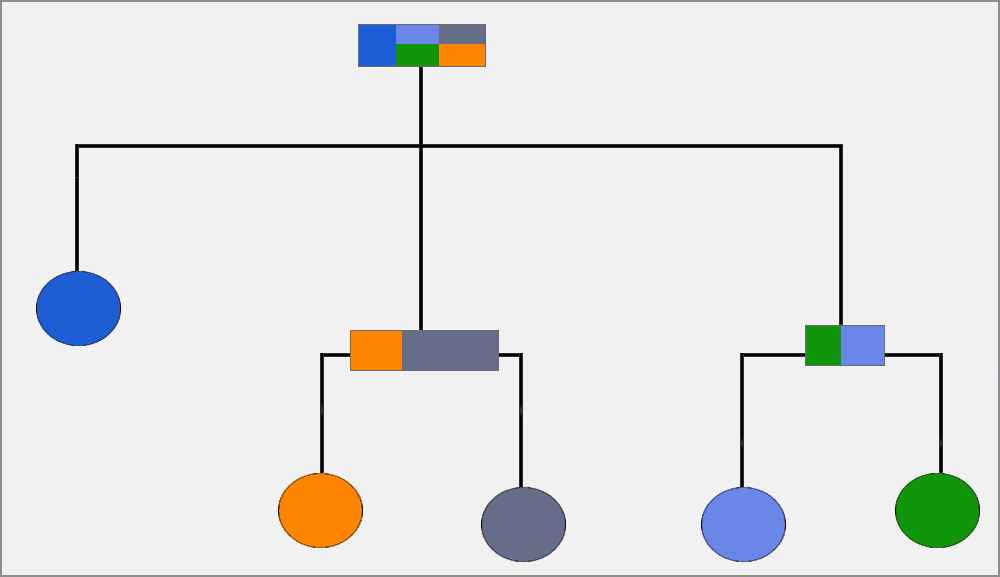
\includegraphics[scale=2]{Images/arbreD.png}
	\caption{Structure d'un arbre de décision}
\end{center}
\label{Arbre}
\end{figure}
A tout arbre de décision est associé une procédure de classification, cette association est définie en parcourant l'arbre de haut en bas, passant par tous les tests menant de la racine à la feuille, qui, une fois atteinte, correspondra à la classe qui sera attribuée à la nouvelle instance.


\newpage
\begin{algorithm}[!h]
\renewcommand\thealgorithm{}
\caption{\textbf{1 } : Algorithme de création d'un arbre de décision}
\begin{algorithmic}
\STATE \textbf{Entrée}:$\tupleset_n=\{t_1,\dots,t_n\}$ ensemble de tuple correspondant au $noeud_n$\\
\textbf{$Arbre A=\{\}$}\\
\textbf{00 : Construction($\tupleset,noeud_n$)}\\
\textbf{01 : DÉBUT}\\
\textbf{02 : }\ \ \ \ \ \ \ \ \ \ \textbf{SI} pour tout tuple $t_i$, $t_i(Y) = y$  \ \ \ \ \  	\textbf{ALORS} \ \ \ \ \ $Nœud_n$ = Feuille(y)\\
\textbf{03 : }\ \ \ \ \ \ \ \ \ \ \textbf{SINON}\\
\textbf{04 : }\ \ \ \ \ \ \ \ \ \ \ \ \ \ \ ChercherAttributDivision($\tupleset)=At_i$\\
\textbf{05 : }\ \ \ \ \ \ \ \ \ \ \ \ \ \ \ Diviser($\tupleset,At_i)=\set X_{ij}$\\
\textbf{06 : }\ \ \ \ \ \ \ \ \ \ \ \ \ \ \ \ \ \ \ \ \ \ \ \ \ \textbf{Répéter(Pour tout n=2 jusqu'à j)}\\
\textbf{07 : }\ \ \ \ \ \ \ \ \ \ \ \ \ \ \ \ \ \ \ \ \ \ \ \ \ \ \ \ \ \ \ \ \ \ \ Créer $noeud_j$\\
\textbf{08 : }\ \ \ \ \ \ \ \ \ \ \ \ \ \ \ \ \ \ \ \ \ \ \ \ \ \ \ \ \ \ \ \ \ \ \ Construction($X_{ij},noeud_j$)\\
\textbf{09 : }\ \ \ \ \ \ \ \ \ \ \ \ \ \ \ \ \ \ \ \ \ \ \ \ \ \textbf{FIN}\\

\textbf{10 : }\ \ \ \ \ \ \ \ \ \ \textbf{FinSI}\\
\textbf{11 : }\ \ \ \ \ \ \ \ \ \ \textbf{$A=\{ A \} \cup Noeud_n$}\\
\textbf{12 : FIN}\\
\textbf{Sortie} : $A$

\label{Algorithme1}
\end{algorithmic}
\addtocounter{algorithm}{-1}
\end{algorithm}


L'algorithme \ref{Algorithme1} représente le déroulement global de la construction d'un arbre de décision, nous remarquons à la ligne 06 qu'à chaque niveau, si le nœud n'est pas homogène, un test doit être choisi afin de diviser l'ensemble de donnée relatif a ce nœud. Le choix du test est considéré comme la partie cruciale de l'algorithme, vu son impacte directe sur l'arbre de décision résultant, ce choix est basé sur des métriques appelées \emph{critères de division}.\\ 

\section{Critères de division}
L'objectif principal d'un critère de division est de maximiser l'homogénéité d'un nœud, et ce, en choisissant l'attribut approprié sur lequel diviser l'ensemble de données.\\
\subsection{Formalisation}
\begin{definition}[Ensemble de tuples homogène]
  Soit $T\subseteq\tupleset$ un ensemble de tuples et soit $Y$ l'attribut de classe.
$T$ est \emph{homogène} si:
$$\forall t, t'\in T, t(Y)=t'(Y)$$
<<<<<<< HEAD
%$\tupleset_{ij}$ est dit homogène si : $\forall{t_j}\forall{t_k} : t_ij(Y) = t_iks(Y)$ 
=======
\end{center}
%$\tupleset_{ij}$ est dit homogène si : $\forall{t_j}\forall{t_k} : t_ij(Y) = t_iks(Y)$ 

\end{definition}
>>>>>>> 351f1cc4c861856cb1444e69f81996a154a06787

\begin{definition}[Division par un attribut et une fonction]
  Soit $T\subseteq\tupleset$ un ensemble de tuples, soit $D$ un ensemble fini et soit $f: \valeurset\rightarrow D$.
  La division de $T$ par $f$ et $X$, notée $division(T,f,X)$ est l'ensemble $\{T_{d_1},\dots,T_{d_n}\}$ tel que:
$$T_{d_i} = \{ t\in T \mid f(t(X)) = d_i \}$$
\end{definition}

\begin{definition}[Division par un attribut et une fonction]
  Soit $T\subseteq\tupleset$ un ensemble de tuples, soit $D$ un ensemble fini et soit $f: \valeurset\rightarrow D$.
  La division de $T$ par $f$ et $X$, notée $division(T,f,X)$ est l'ensemble $\{T_{d_1},\dots,T_{d_n}\}$ tel que:
$$T_{d_i} = \{ t\in T \mid f(t(X)) = d_i \}$$
\end{definition}

\begin{definition}[Critère de division]
%Soit $\tupleset(\attributset, C)$ un ensemble de tuples, caractérisé par : \\
%Soit $\tupleset=t_{i,\dots,n}$ un ensemble de tuples, caractérisé par : \\
Soit $\set{X}$ un ensemble d'attributs et $D$ un ensemble fini.
Un critère de division est de la forme $(eval,choice,homogeneite)$ tel que:
\begin{itemize}
\item $eval: \attributset\rightarrow (\valeurset\rightarrow D)$ associe à chaque attribut une fonction de placement d'une valeur dans un panier.
\item $choice: 2^\tupleset\times 2^\attributset \rightarrow \attributset$ permet de choisir un attribut en fonction d'un ensemble de tuples et d'un ensemble d'attributs.
\item $homogeneite: 2^{2^\tupleset}\rightarrow\real$ définit une notion d'homogénéité sur une partition (résultant d'une division) d'un ensemble de tuples initial.
\end{itemize}
telles que si $choice(T,\set{X}) = X$, et si $f = eval(X)$  alors:
\begin{itemize}
\item $\forall X' $avec $(n',f')=eval(X')$, $homogeneite(division(T,f',X')) \leq homogeneite(division(T,f,X))$
\end{itemize}

% Soit $T\subseteq\tupleset$ un ensemble de tuples et $\set{X}$ un ensemble des attributs.



% On défini les fonctions : \\
% \begin{tabular}{l}
% $chercherAttributDivision(\tupleset,\attributset) = \attributset_i$ \\
% $diviser(\tupleset,\attributset_i) = \set X_{ij(j=2,\dots,n)}$\\
% \end{tabular}
% \\Tel que $\set X_{ij}$ représente les $j$ sous ensembles résultant de la division de $\tupleset$ par rapport à $At_i$\\
% La fonction $chercherAttributDivision$ permet de satisfaire la propriété d'homogénéité, tel que :\\
% $\forall{\set X_{m}} \subset \tupleset, i\neq m, homogeneite(\set X_i\_) \geq homogeinite(\set X_m\_)$
\end{definition}

Il existe plusieurs critères, c'est en grande partie ce qui différencie les algorithmes d'arbres de décision, nous allons détailler les plus utilisés d'entre eux, en utilisant de manière commune le jeu de données suivant :
\begin{figure}[!h]
\begin{center}

\begin{tabular}{| l | l | l | l | l |}
\hline
\rowcolor{gray!25}
Temps & Température & Humidité & Vent & Jouer \\
\hline
Ensoleillé & Haute & Haute & Faux & Non \\
\hline
Ensoleillé & Haute & Haute & Vrai & Non \\
\hline
Couvert & Haute & Haute & Faux & Oui \\
\hline
Pluvieux & Basse & Haute & Faux & Oui \\
\hline
Pluvieux & Moyenne & Normal & Faux & Oui \\
\hline
Pluvieux & Moyenne & Normal & Vrai & Non \\
\hline
Couvert & Moyenne & Normal & Vrai & Oui \\
\hline
Ensoleillé & Basse & Haute & Faux & Non \\
\hline
Ensoleillé & Moyenne & Normal & Faux & Oui \\
\hline
Pluvieux & Basse & Normal & Faux & Oui \\
\hline
Ensoleillé & Basse & Normal & Vrai & Oui \\
\hline
Couvert & Basse & Haute & Vrai & Oui \\
\hline
Couvert & Haute & Normal & Faux & Oui \\
\hline
Pluvieux & Moyenne & Haute & Vrai & Non \\
\hline
\end{tabular}
\caption{Ensemble de données de départ}
\end{center}
\end{figure}
\subsection*{\emph{Gain d'information}}
Le gain d'information est un critère basé sur l'impureté, il utilise l'entropie comme mesure d'impureté (mesure mise au point par \textsc{Quinlan} en 1987)\cite{singh2014comparative}. Dans le cadre de la recherche de l'attribut de division, il correspondra à celui ayant le gain d'information le plus élevé. 

\subsubsection*{Formule}
Le Gain d'information d'un attribut T est égal a la différence entre l'entropie pré-division (nœud père p), et l'entropie post-division (par rapport à l'attribut T), sa formule est la suivante :
\begin{align}
\begin{split}\label{formule:gain}
Gain(p,T) = Entropie(P) - \sum_{j=1}^n (P_j * Log_2(P_j))
\end{split}
\end{align}
\subsubsection*{Exemple}
\begin{itemize}
\item Calcul de l'entropie de l'ensemble\\
Nombre d'instance : 14
\[Nombre \ de catégories \ de \ classe \ : \ 2 \ \left\{ 
\begin{array}{l l}
  Oui : & \quad \text{ 9}\\
  Non : & \quad \text{ 5}\\ \end{array} \right. \]
$Entropie(P) = -((\frac{9}{14})Log_2(\frac{9}{14}) + (\frac{5}{14})Log_2(\frac{5}{14})) = 0.94$
\item Temps

\begin{table}[!h]
\begin{center}
\begin{tabular}{| l | c | c | c |}
\hline
\rowcolor{gray!25}
 & Oui & Non & Nb d'instance\\
 \hline
Ensoleillé & 2 & 3 & 5 \\
\hline
Pluvieux & 3 & 2 & 5\\
\hline
Couvert & 4 & 0 & 4\\
\hline 
\end{tabular}
\caption{Table de comptage de l'attribut Temps}
\end{center}
\end{table}
$Entropie(Temps) = \frac{5}{14}(- (\frac{2}{5} Log_2(\frac{2}{5}) + \frac{3}{5} Log_2(\frac{3}{5}))) + \frac{5}{14}(- (\frac{3}{5} Log_2(\frac{3}{5}) + \frac{2}{5} Log_2(\frac{2}{5}))) + \frac{4}{14}(- \frac{4}{4} Log_2(\frac{4}{4}))\\
Entropie(Temps) = 0.69$
\item $Gain(Temps) = 0.94 - 0.69 = 0.25$
\item Après les calculs :  
\begin{itemize}
\item Gain(Température) = 0.05 
\item Gain(Humidité) = 0.15
\item Gain(Vent) = 0.05
\end{itemize}

L'attribut ayant le gain le plus élevé sera choisi comme attribut de division, ce qui est dans notre exemple l'attribut "Temps"

\end{itemize}

\subsection*{\emph{Rapport du gain d'information}}
Mise au point par \textsc{Quinlan}, le but de ce critre normaliser le Gain d'information, afin palier à la faille de ce dernier, qui a tendance a favoriser les attributs ayant beaucoup de valeur\cite{salzberg1994c4}.

\subsubsection*{Formule}
La mesure \emph{SplitInfo} est utilisée afin de normaliser le Gain d'information, elle représente les informations générées suite a la division de l'ensemble de données d'apprentissage p, en n partitions correspondantes aux différentes valeurs de l'attribut T, la formule est la suivante :
\begin{align}
\begin{split}\label{formule:InfoSplit}
SplitInfo(p,T) = - \sum_{j=1}^n P_j * log_2 (P_j)
\end{split}\\
\begin{split}\label{formule:RapportGain}
GainRatio(p,T) = \frac{Gain(p,T)}{InfoSplit(p,T)}
\end{split}
\end{align}

\subsubsection*{Exemple}
\begin{itemize}
\item Calcul de la mesure InfoSplit\\
\begin{itemize}
\item Temps\\
Nous avons :\\
 

\[Nombre \ de \ modalité \ : \ 3 \ \left\{ 
\begin{array}{l l}
  Ensoleillé : & \quad \text{ 5}\\
  Pluvieux : & \quad \text{ 5}\\ 
  Couvert : & \quad \text{ 4}\\
  \end{array} \right. \]
  
$InfoSplit(Temps) = - (\frac{5}{14}Log_2(\frac{5}{14}) + \frac{5}{14}Log_2(\frac{5}{14}) + \frac{4}{14}Log_2(\frac{4}{14}))\\
InfoSplit(Temps) = 1.577$
\item Après les calculs :
\begin{itemize}
\item InfoSplit(Température) = 1.577
\item InfoSplit(Humidité) = 1
\item InfoSplit(Vent)= 0.98

\end{itemize}

\item Calcul du Rapport de Gain\\
\begin{itemize}
\item $GainRatio(Temps) =\frac{Gain}{InfoSplit} = \frac{0.25}{1.577} = 0.15 $\\ 
Après les calculs :
\begin{itemize}
\item $GainRatio(Température)  = 0.03$  
\item $GainRatio(Humidité)  = 0.15$ 
\item $GainRatio(Vent)  = 0.151$
\end{itemize}
\end{itemize}
Nous remarquons que pour le même jeu de données, le rapport de gain a donné des résultats différents que le gain d'information, par conséquent, l'attribut Temps, au trois valeurs, a été pénalisé, ce qui a donné deux possibilités de choix : Temps, humidité.
\end{itemize}

\end{itemize}


\subsection*{\emph{Le coefficient de Gini}}
Autre mesure de l'impureté, le coefficient de Gini mesure les divergences entre les distributions de probabilité des valeurs de l'attribut cible. Sa valeur varie entre 0 et 1, il est égal à 0 dans une situation d'égalité parfaite entre les individu de l'ensemble, et est égal à 1 dans dans la situation la plus inégalitaire possible. Le coefficient de Gini a été utilisé dans divers travaux, tels que (Breiman et al., 1984) et (Gleanedet al., 1991)\cite{singh2014comparative}
\subsubsection*{Formule}
\begin{align}
\begin{split}\label{formule:Gini}
Gini(S) = 1-\sum\limits_{j=0}^n 1- P_j^2\end{split}
\end{align}

Ou $P_j$ représente la fréquence relative à la classe j dans l'ensemble du nœud père.
\subsubsection*{Exemple}
\begin{itemize}
\item Calcul des coefficients de Gini
\begin{itemize}
\item Gini(Temps = ensoleillé)\\
Nous avons :\\
\[Nombre \ d'instance \ : \ 5 \ \left\{ 
\begin{array}{l l}
  P(vrai) : & \quad \text{ $\frac{2}{5}$}\\
  P(faux) : & \quad \text{ $\frac{3}{5}$}\\ 
  \end{array} \right. \]
\item $Gini(Temps=ensoleillé)= 1 - ((\frac{2}{5})^2 + (\frac{3}{5})^2)=0.48 $\\
\item Après les calculs : 
\begin{itemize}
\item $Gini(Temps = pluvieux) = 1 - ((\frac{3}{5})^2 + (\frac{2}{5})^2)=0.48 $
\item $Gini(Temps = couvert) = 1 - ((\frac{5}{5})^2 =0 $
\item $Gini(Temperature = haute) = 0.5 $
\item $Gini(Temperature = basse) = 0.32 $
\item $Gini(Temperature = moyenne) = 0.39 $
\item $Gini(Humidité = haute) = 0.408 $
\item $Gini(Humidité = normal) = 0.489 $
\item $Gini(Vent = vrai) = 0.5 $
\item $Gini(Vent = faux) = 0.378 $

\end{itemize}
La plus faible valeur du coefficient de Gini correspond au test "Temps=couvert", il sera donc choisi comme attribut de division.
\end{itemize}
\end{itemize}


\subsection*{\emph{Chi-square}}
Le Chi-square est un test statistique, il permet, à partir d'un tableau de contingence, de comparer l'indépendance des variables, afin de savoir si elles sont liées, autrement dis, il permet de vérifier si les distribution des variables différent les unes des autres.

\subsubsection*{Formule}
Le calcule du Chi-square $(X^2)$ repose sur deux tableau, à savoir :
\begin{itemize}
\item Tableau d'observation 
\item Tableau d'estimation 
\end{itemize}

\begin{align}
\begin{split}\label{ChiSquare}
   \chi ^2  = \sum_{i=0}^n \frac{(Observation_i - Estimation_i)^2}{Estimation_i}
\end{split}
\end{align}


\subsubsection*{Exemple}
\begin{itemize}
\item Calcul du $\chi^2$
\begin{itemize}
\item Temps
\begin{itemize}
\item Construction des tables 

\begin{table}[!h]
\begin{small}
\begin{tabular}{cc}

    \begin{minipage}{.5\linewidth}
   
\begin{tabular}{| l | l | l | l | l |}
\hline
\cellcolor{gray!25} & \cellcolor{gray!25}Oui & \cellcolor{gray!25}Non &\cellcolor{gray!25} Total\\
\hline
Ensoleillé & 2 & 3 & 5\\
\hline
Pluvieux & 3 & 2 & 5 \\
\hline
Couvert & 4 & 0 & 4 \\
\hline
Total & 9 & 5 & 14 \\
\hline
\end{tabular} 
      \caption{Tableau d'observation}

    \end{minipage} &

    \begin{minipage}{.5\linewidth}
\begin{tabular}{| l | l | l |}
\hline
\cellcolor{gray!25} & \cellcolor{gray!25}Oui & \cellcolor{gray!25}Non\\
\hline
Ensoleillé & $\frac{5*9}{14} = 3.21$ & $\frac{5*5}{14} = 1.78$\\
\hline
Pluvieux & $\frac{5*9}{14} = 3.21$ & $\frac{5*5}{14} = 1.78$ \\
\hline
Couvert & $\frac{4*9}{14} = 2.57$ & $\frac{4*5}{14} = 1.43$  \\
\hline
\end{tabular} 
      \caption{Tableau d'estimation}
 
    \end{minipage} 
\end{tabular}
\end{small}
\end{table}

\item $\chi^2(Temps)= \frac{(2-3.21)^2}{3.21}+\frac{(3-1.78)^2}{1.78}+\frac{(3-3.21)^2}{3.21}+\frac{(2-1.78)^2}{1.78}+\frac{(4-2.57)^2}{2.57}+\frac{(0-1.43)^2}{1.43}$\\
\end{itemize}
\item $\chi^2(Temps) = 3.55$
\item Après les calculs :
\begin{itemize}
\item $\chi^2(Température) = 0.62$
\item $\chi^2(Humidité) = 2.8$
\item $\chi^2(Vent) = 0.94$
\end{itemize}
\end{itemize}
L'attribut ayant la valeur $\chi^2$ la plus élevée sera choisi comme attribut de division, ce qui est dans ce cas, l'attribut Temps. 

\end{itemize}



\section{Élagage}
Les arbres de décision sont souvent confrontés à deux problèmes, à savoir :
\begin{itemize}
\item La complexité (en terme de taille)\\
Qui se répercute sur l'interprétabilité de l'arbre de décision.
\item Le sur-apprentissage \\
Qui se caractérise par une bonne précision de l'arbre sur l'ensemble d'apprentissage, ainsi qu'une mauvaise sur d'autres ensembles.
\end{itemize}
Afin de palier à ces problème, l'arbre de décision doit être élagué. L'élagage peut se faire de deux manières différentes, pendant la croissance de l'arbre (pre-élagage)ou bien après sa construction (post-élagage)
\\



\subsubsection{Pré-élagage}



Consiste à établir une liste de règles d'arrêt, afin d'empêcher la croissance des branches qui n'améliore pas la précision prédictive de l'arbre\cite{esposito1997comparative}, parmi les réglés d'arrêt nous pouvons citer (entres autres) : 
\begin{itemize}
\item Seuil minimal d'instance
\item Profondeur maximal de l'arbre
\item Se baser sur le test d'indépendance ($\chi^2$)\\
Le $\chi^2$ permet de tester statistiquement l'indépendance d'une variable, le calcul se fait comme suit :\\
\begin{itemize}
\item Calcul du $\chi^1$ 
\item Détermination du DDL (Degré De Liberté)\\
$DDL = (Nombre\ de\ modalité\ d'attribut-1)*(Nombre\ de\ catégorie\ de\ classe)$
\item Déterminer le seuil d'erreur $\alpha$\\
$\alpha$ est un paramètre que l'utilisateur devra choisir, généralement, $\alpha=5\%$
\item A partir de la table statistique dite t table, récupérer la valeur du $\chi_{critique}$, qui correspond à l'intersection des deux valeur, DDL et $\alpha$.
\item Comparer $\chi^2 avec \chi_{critique}$
\begin{itemize}
\item Si $\chi^2 > \chi_{critique}$\\
La distribution de l'attribut est statistiquement non significative.
\end{itemize}
%\multirow{2}{*}{\rotatebox[origin=c]{90}{ CART \ \ \ \ \ \ \ \ \ \ \ \ \ \ \ \ \ \ \ \ \ }}

\begin{figure}[h!]
\begin{center}

%\checkmark & $\times$
\begin{tabular}{| c | c | c | c | c |  c | c | c | c | c | c |}
\hline
&\cellcolor{yellow}$\alpha$  &\cellcolor{yellow} 0.20 &\cellcolor{yellow} 0.15 & \cellcolor{yellow}0.1 & \cellcolor{yellow}0.05 &\cellcolor{yellow} 0.025 &\cellcolor{yellow} 0.01 &\cellcolor{yellow} 0.005 & \cellcolor{yellow}0.001 & \cellcolor{yellow}0.0005\\
\hline
\multirow{5}{*}{\rotatebox[origin=c]{90}{ Degré de liberté $\ \ \ \ \ \ \ $}}& \cellcolor{green}1 & 1.376 &  1.965  & 3.078 & 6.314 & 12.71 & 31.82 & 63.66 & 318.3 & 636.6 \\
&\cellcolor{green} 2 & 1.061 &  1.386  & 1.886 & 2.920 & 4.303 & 6.965 & 9.925 & 22.33 & 31.60 \\
&\cellcolor{green} 3 & 0.978 &  1.250  & 1.638 & 2.353 & 3.182 & 4.541 & 5.841 & 10.21 & 12.92 \\
&\cellcolor{green} 4 & 0.941 &  1.190  & 1.533 & 2.132 & 2.776 & 3.747 & 4.604 & 7.173 & 8.610 \\
&\cellcolor{green} 5 & 0.920 &  1.156  & 1.476 & 2.015 & 2.571 & 3.365 & 4.032 & 5.893 & 6.869 \\
&\cellcolor{green} 6 & 0.906 &  1.134  & 1.440 & 1.943 & 2.447 & 3.143 & 3.707 & 5.208 & 5.959 \\
&\cellcolor{green} 7 & 0.896 &  1.119  & 1.415 & 1.895 & 2.365 & 2.998 & 3.499 & 4.785 & 5.408 \\
&\cellcolor{green} 8 & 0.889 &  1.101  & 1.397 & 1.860 & 2.306 & 2.896 & 3.355 & 4.501 & 5.041 \\
&\cellcolor{green} 3 & 0.883 &  1.100  & 1.383 & 1.833 & 2.262 & 2.821 & 3.250 & 4.297 & 4.781 \\
 \hline

\end{tabular}
\caption{T table}
\end{center}
\end{figure}
\end{itemize}

\begin{comment}
Pour ce, après le calcul du $\chi^2$, nous devons définir une valeur appelé $DDL$ (degré de liberté), qui est calculé à partir de la table d'observation :\\
$DDL = (Nombre\ de\ ligne-1) * (Nombre\ de\ colonne-1)$\\
L'utilisateur devrait fixer un paramètre $\alpha$ appelé "seul d'erreur", généralement, $\alpha$ est fixé à $0.05$.\\

A partir de la table statistique \emph{t table}, faire l'intersection entre la valeur du $DDL$  la valeur $\alpha$, afin d'obtenir le $\chi_{critique}$\\
Si $\chi^2 > \chi_{critique}$ Alors l

Enfin, à partir de la table statistique appelé \emph{t table}, faire l'intersection entre la valeur $\chi^2$ et le valeur du $DDL$, 

\end{comment}
\end{itemize}

\subsubsection{Post-élagage}

Dans ce cas, l'élagage est appliqué à un arbre de décision complètement construit, en supprimant certain sous arabes, dans le but de réduire son taux d'erreur.\\

\begin{paragraph}{Formalisation}

\begin{definition}[Précision d'un arbre de décision]
Soit $\tupleset=\{t_1,\dots,t_n\}$ un ensemble de tuple de test, et soit A un arbre de décision\\
on défini la fonction $precision(A) \in [0,1]$ tel que: \\
$precision(A) = \sum_{i=0}^n \frac{classifie(A,t_i) = t_i(Y)} {t_i(Y)}$
\end{definition}
\begin{definition}[Post-Elagage]

Soit $A=\{a_1,\dots,a_n\}$ un arbre de décision caractérisé par n sous arbres \\
$Pour tout (i=0, \dots, n)$ On défini la fonction : \\
$Elaguer(A,a_i) = A'$, ou $\forall{_{j=0,\dots,n, j \neq i}} A'=\{A\}+a_j,$  Si et seulement si :\\ 

$precision(A') \geq precision(A)$

\end{definition}

\end{paragraph}
L'effet bénéfique de l'élagage a attiré l'attention de nombreux chercheurs, qui ont proposés un certain nombre de méthodes\cite{esposito1997comparative}, parmi ces méthodes nous pouvons citer : \\
\begin{itemize}
\item \emph{REP} : \emph{Reduced Error Prunning}\\
Proposée par \textsc{Quinlan}, et globalement la plus simple a implémenté\cite{quinlan1987simplifying}. elle consiste a découpé le jeu de données en trois parties, deux tiers servirons à la construction de l'arbre, et le tiers restant, appelé "ensemble de test" sera utilisé pour l'élagage.\\
Une fois l'arbre construit, l'élagage se fait comme suit :\\
Au niveau de chaque sous arbre $T'$, l'algorithme compare l'estimation de l'erreur réelle avant et après sa suppression, si la précision de l'arbre ne réduit pas apres suppression de $T'$, ce dernier sera élagué et remplacé par la feuille au nombre d'instance le plus élevé de sa hiérarchie.\\
A noter que l'estimation de l'erreur réelle est calculée avec la formule suivante : \\
\begin{align}
\begin{split}\label{formule:InfoSplit}
Erreur(T) = \frac{Nombre\ d'instance\ mal\ classer}{Nombre\ total\ d'instance}
\end{split}
\end{align}
\end{itemize}






\section{Les algorithmes d'arbre de décision}
Il existe une variété d'algorithme d'arbre de décision, aussi diverse que les critères de division que nous avons citer, nous allons voir avec plus de détails les plus utilisés d'entre eux.
\begin{comment}
La construction des arbres de décision à partir de données n’est pas une discipline nouvelle, la
première apparition remonte à 1963, lorsque les deux statisticiens, MORGAN et SONQUIST, avaient
utilisés des arbres de régression dans un processus de prédiction AID (Automatic Interaction Détection),
ce qui avait ouvert la voie à un ensemble de méthodes, d’abord en 1973 avec THAID (MORGAN
etMESSENGER), ensuite en 1980, avec CHAID (KASS). Néomoins, cette discipline n’a pris de l’ampleur
qu’à partir de 1984, avec l’apparition de la méthode CART (Classification and Regression Tree) de
BREIMAN et al. Ensuite, et grâce à ROSS QUINLAN, qui est considéré comme un des piliers de la discipline,
des méthodes de classifications ont étémisent au point, a commencé par 3, en 1986, ensuite, en
1993, l’amélioration de cette dernière donna naissance à une méthode considérée comme référence
incontournable des arbres de décision, à savoir la méthode C4.5. Cet algorithme à encore évolué en
C5.0 (Sous Unix) et SEE5 (Sous Windows), mais en étant cette fois ci implémentée dans un logiciel
commercial[chen1996data].
\end{comment}

\begin{figure}[!h]
\begin{center}
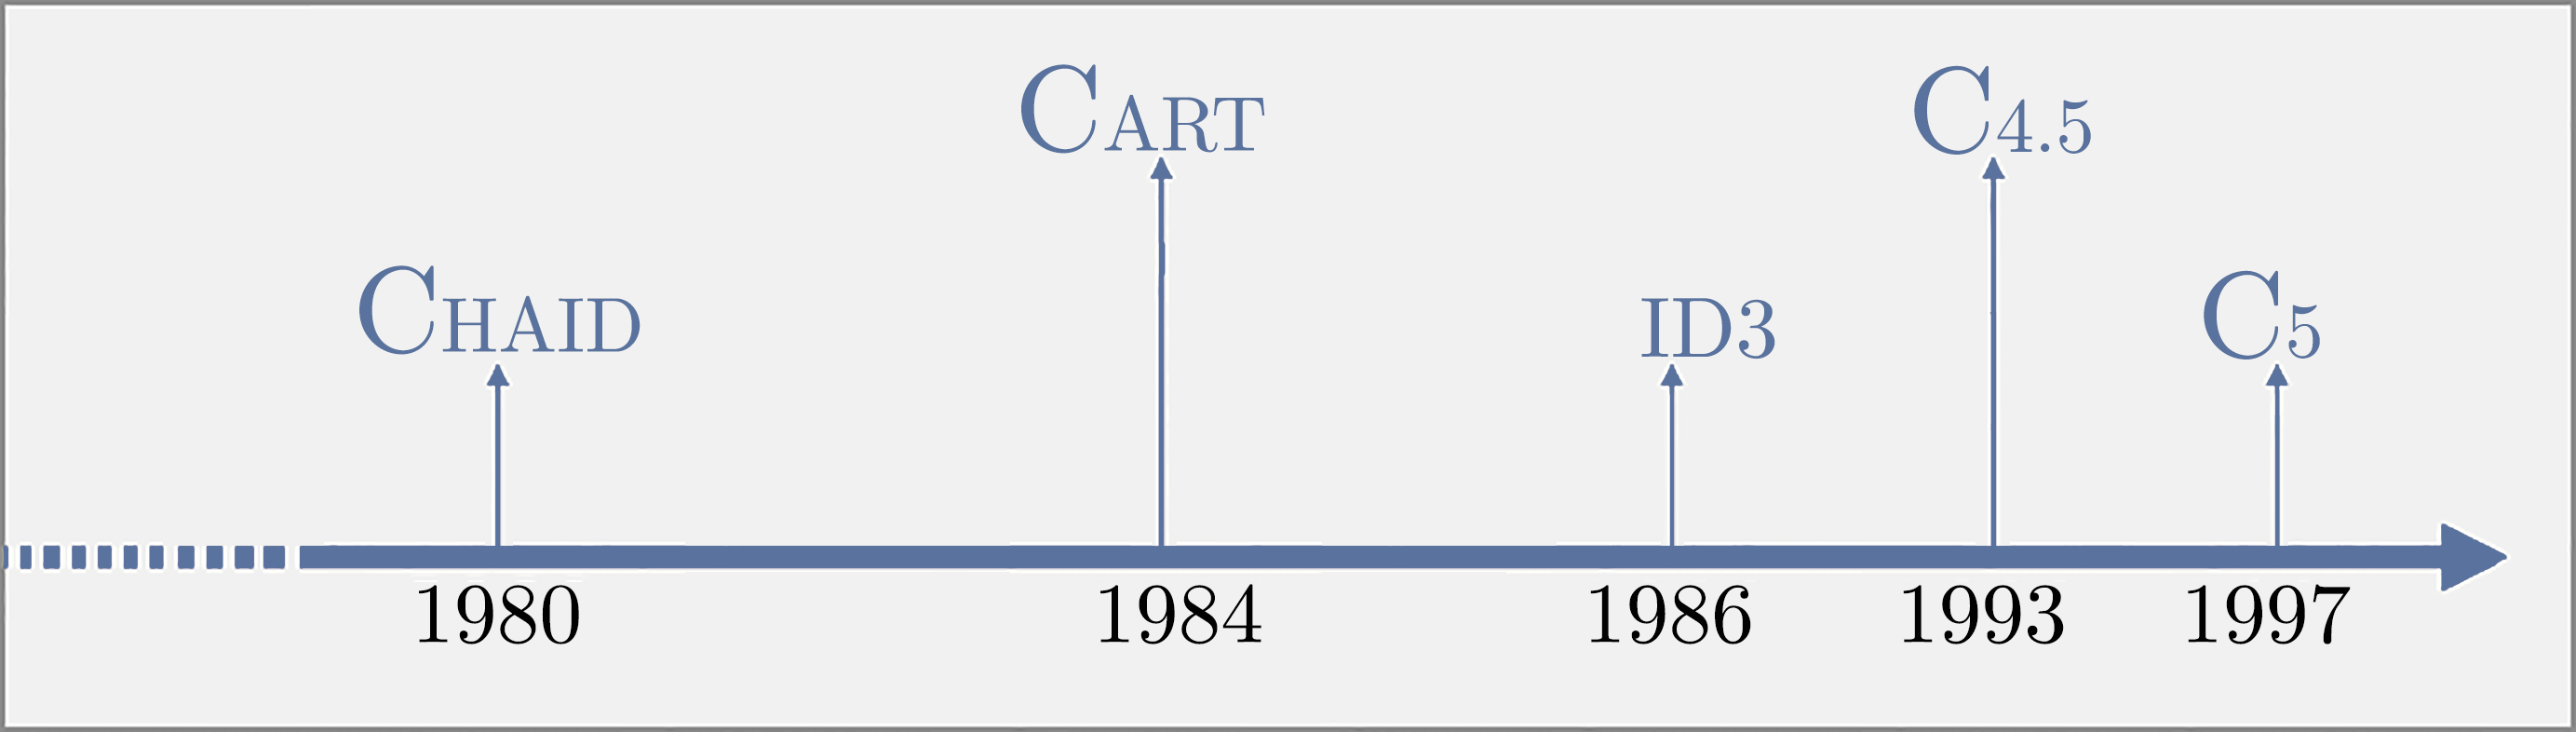
\includegraphics[scale=0.3]{Images/Historique}
\caption{Apparition des algorithmes d'arbre de décision par ordre chronologique}
\end{center}
\end{figure}


\subsection{\emph{CHAID : Chi-Squared Automatic Interaction Detection}} 
Un des plus anciens algorithmes d'arbres de décision, proposés en 1980 par \textsc{Kass}. \\
Comme son nom l'indique, cet algorithme utilise le test du $\chi^2$ comme critère de division\cite{wilkinson1992tree}. En dépit de la puissance et de la robustesse du $\chi^2$, son aspect statistique rend la qualité des résultats relative au volume de données d'apprentissage, en d'autres termes, CHAID est beaucoup plus adapté aux grands qu'aux petits volume de données.\\
Il utilise le pré-élagage en se basant sur le test d'indépendance $\chi^2$, afin de déterminer si le test est statistiquement signifiant ou pas.
\begin{figure}[h!]
\begin{center}
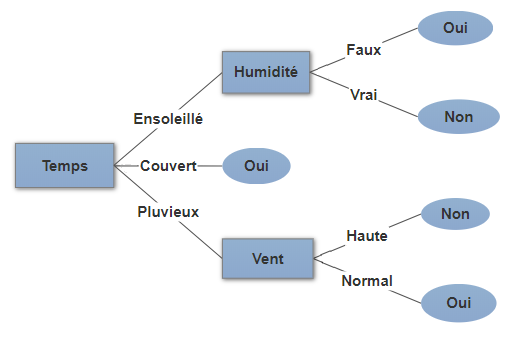
\includegraphics[scale=0.55]{Images/arbre_id3}
\end{center}
\caption{Exemple d'arbre de décision crée en utilisant CHAID}
\end{figure}

\begin{comment}

Le seul paramètre qui permet à l’utilisateur d’intervenir, est bien sûr le choix du seuil d’erreura . Ce paramètre peut être un avantage du fait qu’il permet d’ajuster l’algorithme et de le contrôler suivant par exemple, le domaine étudié et les résultats souhaités. Mais d’un autre coté, il peut poser un autre problème, du fait qu’un mauvais choix de ce paramètre, peut conduire à des résultats inexplicables. Donc la présence d’un expert humain est un atout exigé.

\end{comment}

\subsection{\emph{CART : Classification and Regression Trees}} 
Mis au point par le statisticien \textsc{Leo Breiman} en 1984, il est considéré comme une des références incontournable des arbres de décision. \emph{CART} utilise \emph{le coefficient de Gini} comme critère de division, cette dernière est de type binaire, chaque test partitionne l'ensemble de données en deux sous ensemble, ceux pour lesquels la réponse est positive et négative. L'arbre obtenu est ensuite élagué en utilisant la méthode post-élagage \emph{CCP} (\emph{Cost–Complexity Pruning}.\\
CART peut gérer tout types d'attribut (continu ou discret) ainsi que des instances a valeur manquante ou aberrantes\cite{Hssina2014ACS}.
\begin{figure}[h!]
\begin{center}
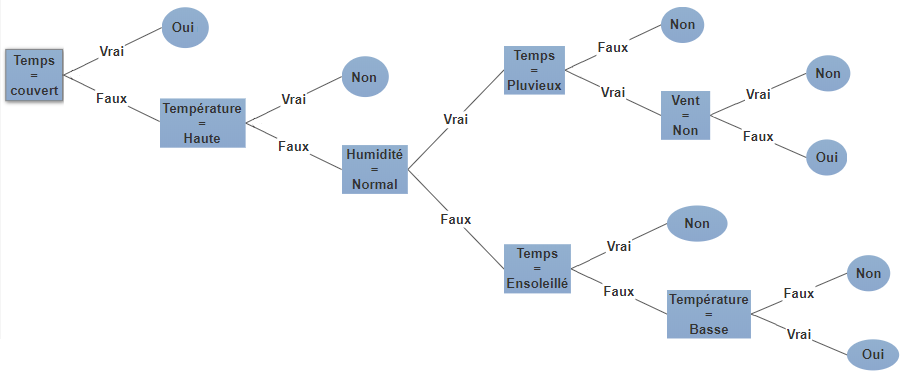
\includegraphics[scale=0.55]{Images/arbre_cart2}
\end{center}
\caption{Exemple d'arbre de décision crée en utilisant CART}
\end{figure}



\subsection{\emph{ID3 : Iterative DiChaudomiser 3}} 
Mise au point par \textsc{Ross Quinlan} en 1986, après l'avoir publié en 1975 dans un libre intitulé « Machine Learning ». Parmi les plus simples des algorithmes d'arbres de décision. \\Il utilise le Gain d'information comme critère de division, il ne gère que les attributs discrets ainsi que des instances à valeurs connues\cite{Hssina2014ACS}.\\ID3 utilise la méthode pre-élagage du test d'indépendance $\chi^2$, avec comme condition que l'attribut soit statistiquement significatif afin d'être sélectionné comme attribut de division.
\begin{figure}[h!]
\begin{center}
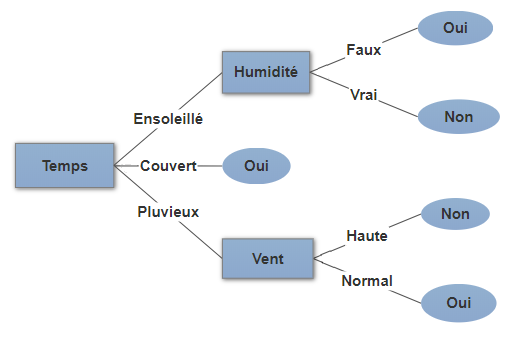
\includegraphics[scale=0.55]{Images/arbre_id3}
\end{center}
\caption{Exemple d'arbre de décision crée en utilisant ID3}
\end{figure}
%%%%

\subsection{C4.5} 

Proposé en 1993 par le même \textsc{Ross Quinlan}, comme amélioration de son premier algorithme (ID3). C4.5 se base sur le Rapport de Gain comme critère de division. L'arbre de décision crée sera ensuite élagué en utilisant la méthode \emph{EBP (Error-Based Pruning)}\cite{quinlan2014c4}. Les améliorations apportées (par rapport à ID3) sont les suivantes\cite[pandya2015c5] :
\begin{itemize}
\item Gestion des attribut continus\\
Tâche réalisée en quatre temps :
\begin{enumerate}
\item Trier les valeurs de l'attribut par ordre croissant.
\item Créer un seuil pour chaque couple de valeurs consécutives $(A = \frac{Val1 + Val2}{2})$. 
\item Pour chaque seuil :
\begin{itemize}
\item Rendre la liste des attributs ayant une valeur supérieur et inférieur ou égal au seuil
\item Calculer l'information apportée par l'attribut.
\end{itemize}
\item Le seuil qui apportera le maximum d'information sera choisi.
\end{enumerate}
\item Gestion des attributs aux valeurs manquantes\\
\end{itemize}
\begin{figure}[h!]
\begin{center}
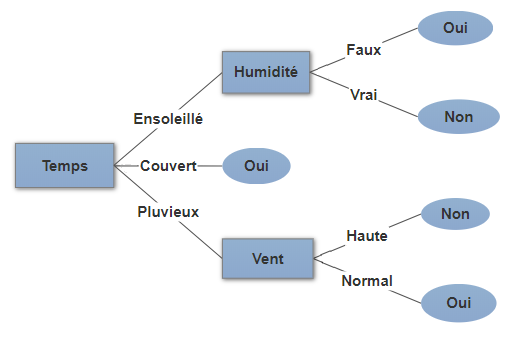
\includegraphics[scale=0.55]{Images/arbre_id3}
\end{center}
\caption{Exemple d'arbre de décision crée en utilisant C4.5}
\end{figure}
\begin{comment}
En fait, les arbres de décision comme les arbres C4.5 et CART étaient parmi les premiers algorithmes qui incorporent la manipulation des données manquantes dans l'algorithme lui-même.
La gestion des données manquantes dans les arbres de décision pose trois problèmes:
a) Comment peut-on affecter la présence de données manquantes? Le processus de choix du meilleur candidat-test
b) une fois qu'un test est sélectionné, que faire des instances qui ont des valeurs manquantes sur la variable de test
c) au moment de la prédiction comment procéder avec une instance qui doit être testée par rapport à une variable qui a une valeur manquante pour l'instance donnée

Ce que spécifie C4.5 est décrit pour chaque problème.

a) Test d'évaluation
C4.5 peut utiliser InfoGain ou GainRatio. InfoGain est le gain en entropie après qu'un test divise des données.
Il peut être noté que pour les étiquettes manquantes sur les colonnes de test, ces instances ne produiront aucun gain d'information. 
Ainsi, s'il y a des données manquantes 
InfoGain = p * (OldEntropy-NewEntropy) + (1-p) * 0 = p * (OldEntropy-NewEntropy), 
où p est la fraction d'instances avec des valeurs complètes non manquantes. Pour ammend la formule pour GainRation,
vous devez également noter que pour les données manquantes apparaît comme une nouvelle catégorie dans la formule de SplitInfo, donc il y a n + 1 groupes de données.
..
b) Partitionner l'ensemble d'entraînement
Après avoir choisi un test, les instances sont divisées en deux ou plusieurs groupes, un groupe pour chaque nœud. Évidemment,
pour les instances avec des données manquantes sur la variable de test, nous n'avons aucun critère pour choisir le nœud. Ce que C4.5 propose est d'envoyer toutes les instances avec une valeur manquante sur la variable de test à envoyer à tous les nœuds enfants,
mais avec un poids diminué par la multiplication avec la proportion égale à la proportion d'instances de ce nœud enfant du nombre total d'instances non manquantes. Par exemple vous avez une colonne de test Sex avec 10 instances ayant 'male', 30 instances ayant 'female' et 5 instances ayant une valeur manquante.
Les 5 occurrences manquantes seront envoyées aux nœuds des deux sexes, avec des poids multipliés par 10/40 pour les ados «mâles» 30/40 pour les nœuds «femelles».
.
.
.
c) Instances de prévision avec des valeurs manquantes. Quand au moment de la prédiction nous rencontrons un nœud dans l'arbre de décision qui teste une variable A,
et pour cette variable nous avons dans notre exemple une valeur manquante que toutes les possibilités sont explorées. Ainsi, pour chaque sous-noeud possible, une prédiction est faite. Nous conservons la distribution pour chaque sous-noeud et nous les ajoutons. Enfin, la classe choisie pour la prédiction est la classe avec la plus grande valeur de densité.


\end{comment}
\newpage
\subsection{C5} 
Une amélioration de l'alorithme C4.5, mis au point en 1997 par le même \textsc{Ross Quinlan}. \\Etant une version commerciale, les détails de l'implémentation n'ont pas tous été révélés, neaumoins, à travers ce qui à été publié, nous pouvons énumérer les améliorations suivantes\cite{wu2008top} :\\
\begin{itemize}
\item Utilise l'apprentissage ensembliste\\
Qui consiste à partitionner les données d'apprentissage et de créer un modèle relatif à chaque partie. L'ensemble des modèles sera utilisé lors de la classification, et se, en faisant l'agrégation de leurs résultat.
\item Nouveau type de données (heure, date)
\end{itemize}
Le coté technique a aussi été amélioré, parmi les points fort du C5 (par rapport au C4.5)\cite{pandya2015c5} : 
\begin{itemize}
\item Rapidité
\item Faible utilisation de la mémoire
\item Meilleur taux de précision
\end{itemize}
\newpage
\subsection{Récapitulatif}
\begin{table}[h!]
\begin{center}
\begin{tabular}{|c|L{2cm}|L{2cm}|L{2cm}|L{2cm}|L{2cm}|}
\hline
\rowcolor{gray!25} &CHAID&CART&ID3&C4.5&C5\\
 \hline
\cellcolor{gray!25}\rotatebox[origin=c]{90}{ Critère de division }
 &
$\chi^2\ (Chi-square)$
 &
Coefficient de Gini
 &
Gain d'information
 &
Rapport du gain
 &
Rapport du gain
  \\
  \hline
 \cellcolor{gray!25} \rotatebox[origin=c]{90}{ Type de division }
 &
Multiple
 &
Binaire
 &
Multiple
 &
Multiple   
 &
Multiple 
  \\
    \hline

 \cellcolor{gray!25} \rotatebox[origin=c]{90}{ Type d'attribut }
 &
Discrets et continus
 &
Discrets et continus
 &
Discrets
 &
Discrets et continus
 &
Discrets et continus
  \\
    \hline

\cellcolor{gray!25}  \rotatebox[origin=c]{90}{ Élagage }
 &
Pre-élagage :\newline 
test du $\chi^2$
 &
Post-élagage :\newline
Cost Complexity Pruning
 &
Pre-élagage :\newline
test du $\chi^2$
 &
Post-élagage :\newline
Error-Based Pruning
 &
Binomial Confidence Limit
  \\
    \hline
\cellcolor{gray!25}  \rotatebox[origin=c]{90}{ Valeur manquante }
 &
Oui
 &
Oui
 &
Non
 &
Oui
 &
Oui
  \\
    \hline
\end{tabular}
\caption{Récapitulatif des fonctionnalités de chacun des algorithmes}
\end{center}
\end{table}
\subsection{Comparaison}
%utiliser un algorithme avec un jeu  de donné nn approprié, qui lu ies tnn app
%pourrais comprometre la qualité
La recherche faite nous emmène à déduire que la force de chacun de ces algorithmes est relative à un contexte particulier, qui est le jeu de données d'apprentissage, la comparaison entre algorithmes ne peut donc se faire qu'en fonction de ce contexte.\\
Rappelons que dans les arbres de décision, le modèle est crée qu'en faisant la correspondance entre les entrées et les sorties des instances d'apprentissage, ce modèle aura donc +/- la même qualité que celle de l'ensemble de données utilisé. Cet ensemble peut être défini par le biais d'un ensemble de paramètres, tel quel : 
\begin{itemize}
\item Taille\\
Qui est exprimée en nombre d'instance, elle varie d'un type de traitement à un autres, selon l'ampleur de ce dernier.
\item Attribut \\
Plusieurs critères peuvent être associés aux attributs : 
\begin{itemize}
\item Nombre d'attribut
\item Nombre de modalité d'attribut
\item Type d'attribut (continu ou discret)
\end{itemize}
\item Classe\\
Qui correspond à l'attribut à prédire, elle est défini par : 
\begin{itemize}
\item Un nombre de catégorie\\
Qui peut être binaire ou N-aire.
\item Type\\
Qui, dans le cas d'une classification, sera de type discret, et dans le cas d'une régression, sera de type continu.
\end{itemize}
\end{itemize}
C'est à travers ces caractéristiques que les performances des algorithme peuvent être mesurées, à l'aide de plusieurs métriques, telles que : \\
\begin{itemize}
\item Précision\\
Représente un ratio entre le nombre de prédiction bien faite, et le nombre total de prédiction, ce ratio est estimé à partir de l'ensemble de test, qui n'à pas été utilisé lors de l'apprentissage.
\item Complexité\\
Représente la taille de l'arbre de décision conçu, il peut être mesure en nombre de nœud, ou en profondeur de l'arbre.
\item Temps d'exécution\\
Représente le temps écoulé lors de la création du modèle ou lors de la classification.
\end{itemize}
Lors de la création d'un modèle, il est très important d'utiliser les courbes, dites "courbes d'apprentissage", afin de suivre ces performances. et ce, dans le but de mieux estimer les caractéristiques qui lui seront adéquates. 

\begin{figure}[h!]
\begin{center}
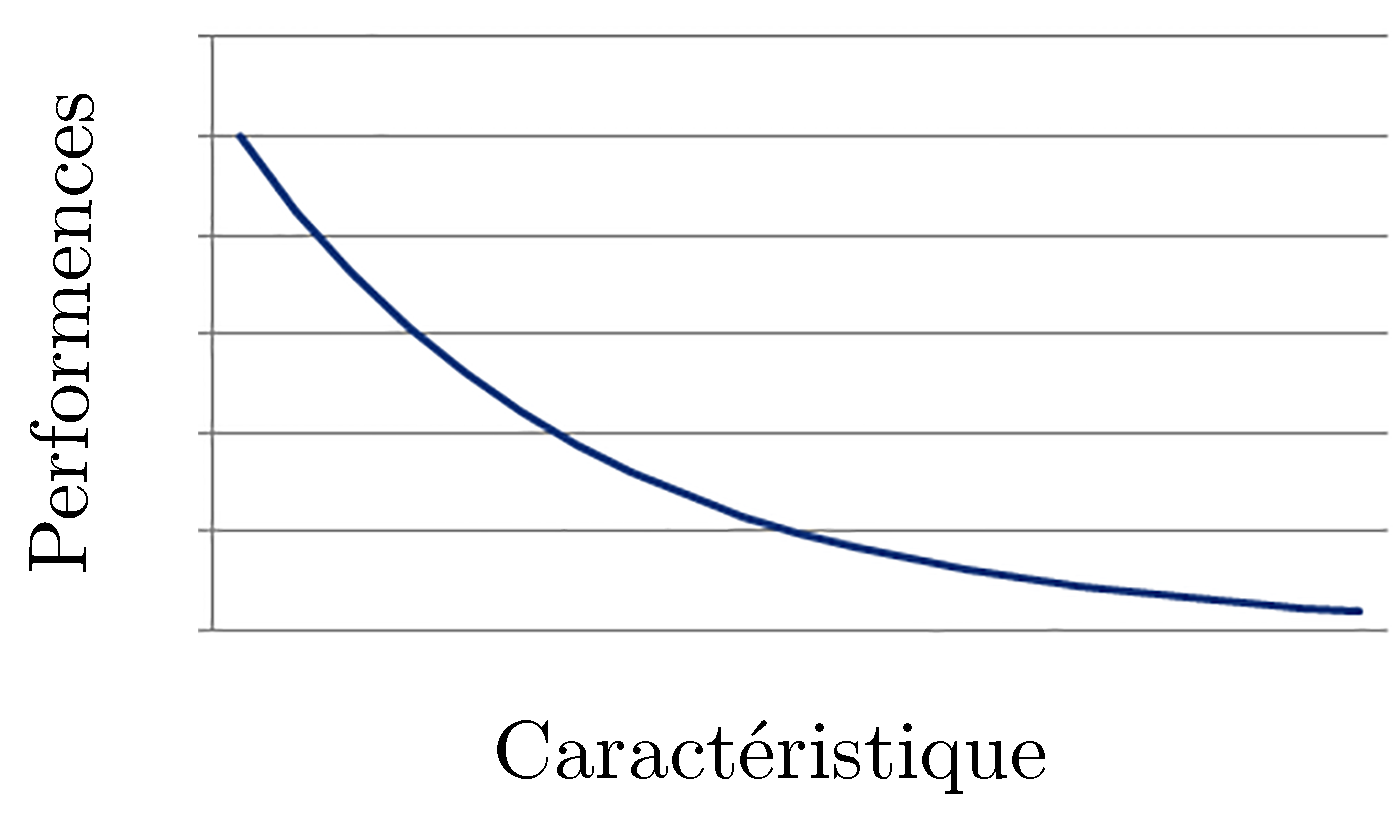
\includegraphics[scale=0.5]{Images/courbe}
\caption{Courbe d'apprentissage}
\end{center}

\end{figure}
Nous allons voir, à travers le tableau ci-dessous, quels sont les conditions appropriées pour chacun des algorithmes vu précédemment.
\newpage
\begin{figure}[h!]
\begin{center}
%\checkmark & $\times$
\begin{tabular}{|c|L{3cm}|L{3cm}|L{3cm}|}
\hline
&Taille & Attribut & Classe \\
 \hline
\multirow{2}{*}{\rotatebox[origin=c]{90}{ CHAID \ \ \ }}&\cellcolor{gray!25}Précision \checkmark & \cellcolor{gray!25}Temps $\times$ & \cellcolor{gray!25}Temps $\times$\\
&Adapté au grand volume de données & Non adapté au grand nombre de modalité d'attribut, car :\newline ça fera augmenter le nombre de ligne de la table de contingence & Non adapté au grand nombre de catégorie de classe, car :\newline ça fera augmenter le nombre de colonne de la table de contingence\\
 \hline
\multirow{2}{*}{\rotatebox[origin=c]{90}{ CART \ \ \ \ \ \ \ \ \ \ \ \ \ \ \ \ \ \ \ \ \ }}&\cellcolor{gray!25} $ \ \ \ \ \ \ \ \ \ \ \ \  $  \checkmark  & \cellcolor{gray!25}Complexité $\times$& \cellcolor{gray!25}Complexité\checkmark\\
&Indifférent à la variation de taille, car : \newline Sa formule est légère & Non adapté au grand nombre de modalité d'attribut, Car :\newline Son critère divise par valeur d'attribut et non par attribut& Adapté aux classes à catégorie binaire\\
  \hline
\multirow{2}{*}{\rotatebox[origin=c]{90}{ ID3 \ \ \ \ \ \ \ \ \ \ \ \ \ \ }}&\cellcolor{gray!25} Temps $\times$ & \cellcolor{gray!25}Complexité $\times$& \cellcolor{gray!25} $ \ \ \ \ \ \ \ \ \ \ \ \  $\checkmark \\
&Non adapté au très grand volume, à cause :\newline Des logarithmes utilisés dans le calcule du gain & 

Non adapté au nombre réduit de modalité, car :\newline il utilise le Gain d'information comme critère de division \newline
Non adapté aux attributs de type continu

 & Indifférent à la variation de la classe\\
  \hline
\multirow{2}{*}{\rotatebox[origin=c]{90}{ C4.5 \ \ \ \ \ \ \ \ \ \ \ \ \ \ }}&\cellcolor{gray!25} Temps $\times$  & \cellcolor{gray!25}Complexité \checkmark &\cellcolor{gray!25} $ \ \ \ \ \ \ \ \ \ \ \ \  $\checkmark \\
& Non adapté au très grand volume, du au calcul : \begin{itemize}
\item Gain
\item InfoSplit
\end{itemize}  & Adapté au nombre élevé de modalité (grâce du Rapport de gain) & Indifférent à la variation de la classe\\
  \hline
\end{tabular}
\end{center}
\end{figure}




\section{Conclusion}

............................................................\\
............................................................\\
............................................................\\

\end{chapter}
\printbibliography 
\end{document}
